\documentclass{article}

%\usepackage{psfig}

\setlength{\evensidemargin}{0in} \setlength{\oddsidemargin}{0in}
\setlength{\textwidth}{6.7in} \setlength{\topmargin}{-1.1in}
\setlength{\textheight}{10.5in}


\usepackage{amssymb, amsthm, amstext, amsxtra, amsmath, amsfonts, amscd }
\usepackage{graphicx, epsfig}
\usepackage{comment}
\usepackage{color}
\usepackage{cleveref}
\usepackage{listings}
 
% Code colors

\definecolor{dkgreen}{rgb}{0,0.6,0}
\definecolor{gray}{rgb}{0.5,0.5,0.5}
\definecolor{mauve}{rgb}{0.58,0,0.82}
\definecolor{backcolour}{rgb}{0.95,0.95,0.92}

\lstdefinestyle{mystyle}{
frame=tb,
backgroundcolor=\color{backcolour},
language=R,
aboveskip=3mm,
belowskip=3mm,
showstringspaces=false,
columns=flexible,
numbers=none,
keywordstyle=\color{blue},
numberstyle=\tiny\color{gray},
commentstyle=\color{dkgreen},
stringstyle=\color{mauve},
breaklines=true,
breakatwhitespace=true,
tabsize=3
}
\lstset{style=mystyle}


\def\E{\mathbb{E}}
\def\pr{\mathbb{P}}

\renewcommand\baselinestretch{1.2}

\DeclareMathOperator{\sign}{sign}
\DeclareMathOperator{\supp}{supp}

\DeclareMathOperator{\Cov}{Cov}
\DeclareMathOperator{\Var}{Var}
\DeclareMathOperator{\corr}{corr}


\author{Salvador Garcia, s1655274}

\date{27 January 2016}


\title{Assgn1: Student's goals}

\begin{document}

\maketitle
%\tableofcontents
%\newpage

\section{Description of the problem} 

229 students (109 boys and 120 girls) aged 7-13 from 9 schools were asked whether popularity or sporting ability was most important to them. The outcome is summarized in
the table below. The question is to determine whether there is a difference between the
importance of popularity and of sporting ability for girls and boys.

\begin{table}[h]
\centering
\begin{tabular}{l|cc|}
\cline{2-3}
                            & \multicolumn{1}{l|}{Sporting ability} & \multicolumn{1}{l|}{Popularity} \\ \hline
\multicolumn{1}{|l|}{Boys}  & 59                                    & 50                              \\
\multicolumn{1}{|l|}{Girls} & 30                                    & 90                              \\ \hline
\end{tabular}
\end{table}

\section{Likelihood}  
Introduce the following random variables. Consider the $i$th boy, $i = 1,2, ..., n = 109$, and set $X_i = 1$ if popularity is more important to him than sports, and $X_i = 0$ otherwise. Similarly, for the $j$th girl, $j = 1,2, ...,m = 120$, set $Y_j = 1$ if popularity is more important to her than sports, and $Y_j=0$ otherwise.
Possible likelihood (independently $\theta_1$ and $\theta_2$ respectively):

\begin{equation}
\begin{split}
X_i | \theta_1  \thicksim& Bern(\theta_1),\quad \theta_1 \in (0,1), i = 1,2,...,n\\
Y_i | \theta_2  \thicksim& Bern(\theta_2),\quad \theta_2 \in (0,1), i = 1,2,...,m
\end{split}
\end{equation}

Also, $X_i$ and $Y_j$ are independent for all $i, j$. This data, can be summarized as a binomial variable, with two parameters $n$ and $p$ with the next distributions:

\begin{equation}
\begin{split}
S_X = \sum_i^n X_i  \thicksim&  Bin(n, \theta_1) \\
S_Y = \sum_i^m Y_i  \thicksim&  Bin(m, \theta_2) \\
\end{split}
\end{equation}

As $S_X$ and $S_Y$ are sufficient statistics for the binomial distribution, then there is no loss of information of $\theta_1$ and $\theta_2$ respectively. Now, $\theta_1$ and $\theta_2$ can be estimated as:

\begin{equation}
\begin{split}
\widehat{\theta}_1 = \frac{\sum_i^n X_i}{n}\\
\widehat{\theta}_2 = \frac{\sum_i^m Y_i}{m}
\end{split}
\end{equation}

As can be seen from the above formulas, the parameters $\theta_1$ and $\theta_2$ are the average of the outcomes $X_i$ and $Y_i$ respectively. Then, used in the binomial distribution, this is the probability that boys or girls prefer popularity over sporting ability. In order to discover if there is a difference between the preferences of the preferences of boys and girls, one option is to test the hypothesis $\theta_1 = \theta_2$ or equivalently, $\theta_1 - \theta_2 = 0$.

In this example, the values of the MLE of $\theta_1$ and $\theta_2$ can be calculated with the next expressions: $\sum_i^n X_i = 50$ and $\sum_i^n Y_i = 90$, $m = 120$, $n = 109$. 

\section{Prior distribution}	
\subsection{Available prior information}

The binomial distributions is made with two parameters: $n$ and $p$. The first is the number of trials and the second the probability of success. The number of trials for $\theta_1$ and $\theta_2$ is determined by $n$ and $m$ and are known. Now, the problem is to estimate $p$. For this section three prior distributions for $\theta_1$ will be considered. The first two are not informative priors: the first is an uniform distribution over $[0,1]$, the second the Jeffrey's prior for the binomial likelihood. The last one, is a informative prior that was obtained from a previous study. For the $\theta_2$, only two priors will be considered and are the same non-informative priors used for $\theta_1$. 

The informative prior that is used in this example has important implications. It is stated that this distribution is the posterior distribution made from a \textit{boys-only school}. It is not stated when this study was made, so there could be a bias because of the year of study. Generations change between each other in the time. Another bias that can be introduced from this posterior distribution is that the school is a $boys-only$ school, so each boy have only contact with more boys, so the perception of popularity and sport ability could be different. The third factor of bias is that it is not stated if the where was this school or if this was a private or public school. Such differences can potentially bias the study. So make the assumption that is the same population could be dangerous.

\subsection{Prior distribution(s)}

The following two uninformative prior distributions can be used for the distribution:

\begin{centering}
\begin{enumerate}
	\item{$p(\theta_i) = 1$, $\theta_i \in [0,1]$}
	\item{$\theta \thicksim beta(1/2, 1/2)$}
\end{enumerate}
\end{centering}

Like $\widehat{\theta}_i$ is a probability, its range is between $0$ and $1$. Then, a uniform distribution can be used for this example. The second one is the Jeffrey prior for $\theta_i$.

This Jeffrey prior can be derived as follows:

\begin{equation}
\begin{split}
	p(x|\theta_i) =& {n\choose x} \theta_i^x (1- \theta_i)^{n-x} \\
	\log p(x|\theta_i) =& \log {n\choose x} + x \log \theta_i + (n-x) \log (1-\theta_i) \\
\end{split}
\end{equation}

Then deriving with respect $\theta_i$:

\begin{equation}
\begin{split}
	\frac{d \log p(x|\theta_i)}{d\theta_i} =& +\frac{x}{\theta_i} - \frac{(n-x)}{(1-\theta_i)} \\
	\frac{d^2 \log p(x|\theta_i)}{d\theta_i^2} =& -\frac{x}{\theta_i^2} - \frac{(n-x)}{(1-\theta_i)^2} 
\end{split}
\end{equation}

Finally, $E_{\theta_i}(x) = n\theta_i$ so:

\begin{equation}
\begin{split}
	-E_\theta\left(\frac{d^2 \log p(x|\theta_i)}{d\theta_i^2}\right) =& \frac{n\theta_i}{\theta_i^2} + \frac{(n-n\theta_i)}{(1-\theta_i)^2} \\
	=& \frac{n}{\theta_i} + \frac{(n)}{(1-\theta_i)} \\
	=& \frac{n}{\theta_i(1-\theta_i)}
\end{split}
\end{equation}

\newpage

Taking square root, the last expression is proportional to $\theta_i^{-\frac{1}{2}}(1-\theta_i)^{-\frac{1}{2}}$ i.e. equivalent to the kernel of a beta distribution with parameters $(\frac{1}{2}, \frac{1}{2})$.

The third prior to be used will be an informative one, this is the posterior distribution obtained from a previous analysis. The school was a boys-only school and this distribution is a \textit{Beta(21,10)}. 

\begin{figure}[ht!]
    \centering
    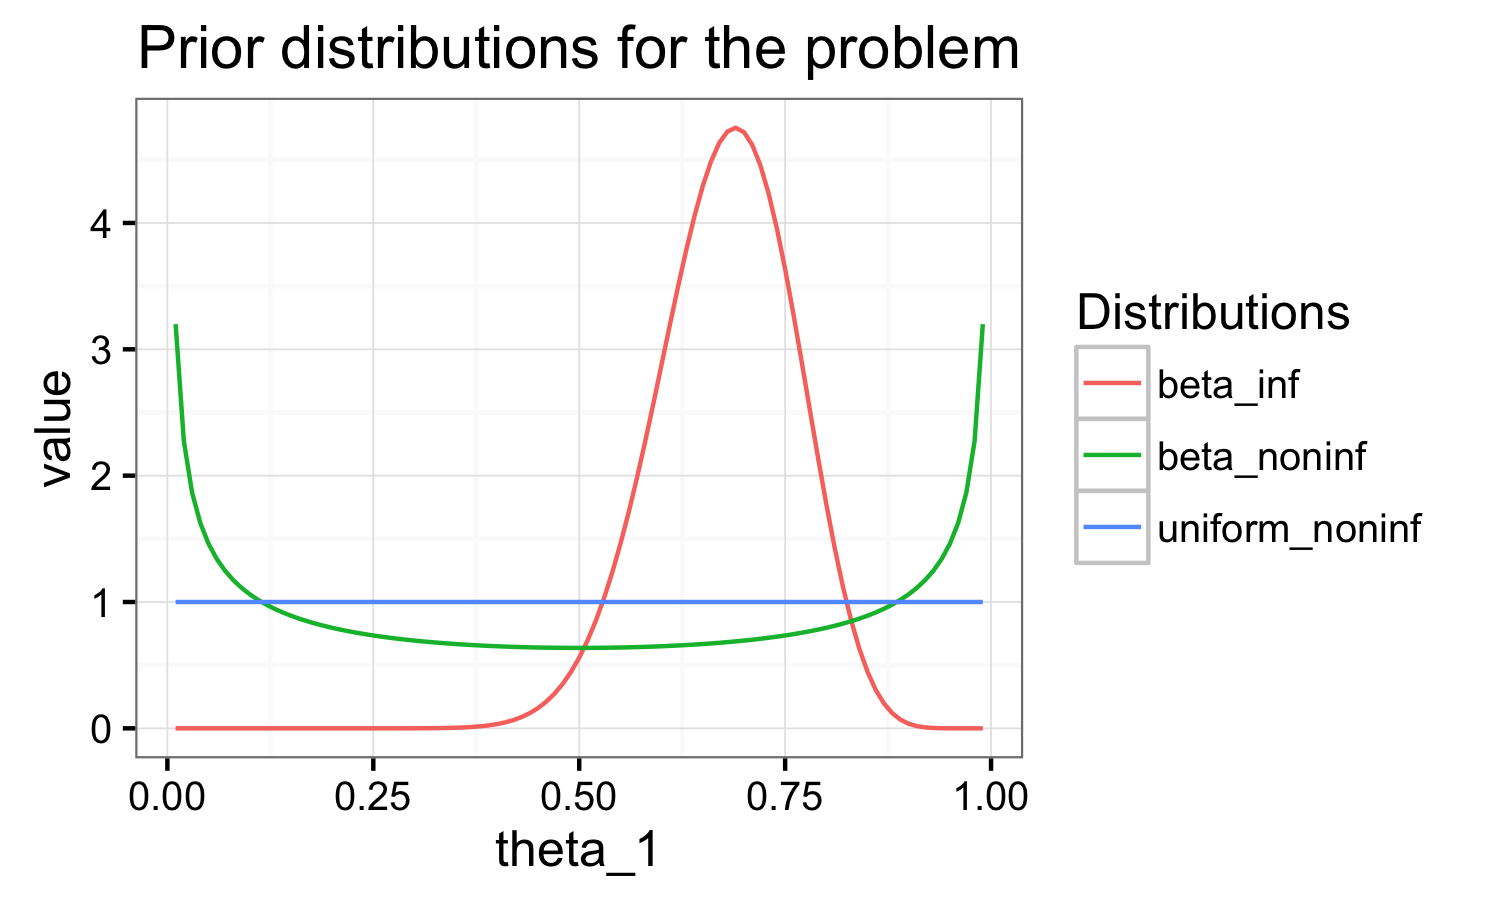
\includegraphics[scale=.20]{11_Assignment1/priors_dist.png}
    \caption{Priors distributions used for the study}
    \label{fig:fig1}
\end{figure}


\section{Posterior inference}	

The prior distribution will be represented as $p(\theta_i)$ with $i = 1,2$. Then, the likelihood is a binomial distribution that can be written as (with $\bar{X}$ the sample):

\begin{equation}
	p(\bar{X}|\theta_i) \propto \theta_i^{\sum_{X_i}} (1- \theta_i)^{n-\sum_{x_i}}
\end{equation}

Then, for the first prior (uniform), the posterior takes this form:

\begin{equation}
\begin{split}
	p(\theta_i|\bar{X}) \propto& \theta_i^{\sum_i X_i} (1- \theta_i)^{n-\sum_i x_i}\\
	\propto& \theta_i^{50} (1- \theta_i)^{59}
\end{split}
\end{equation}

That is the kernel of a $Beta(51, 60)$. For the second prior distribution (Jeffrey's prior), the posterior takes the form:

\begin{equation}
\begin{split}
	p(\theta_i|\bar{X}) \propto& \theta_i^{\sum_i X_i-\frac{1}{2}} (1- \theta_i)^{n-\sum_{x_i}-\frac{1}{2}} \\
	\propto& \theta_i^{49.5} (1- \theta_i)^{58.8}
\end{split}
\end{equation}

That is the kernel of a $Beta(50.5, 59.5)$. For the last prior distribution (Informative), the posterior distribution takes the form:

\begin{equation}
\begin{split}
	p(\theta_i|\bar{X}) \propto& \theta_i^{\sum_i X_i+21} (1- \theta_i)^{n-\sum_{x_i}+10} \\
	\propto& \theta_i^{71} (1- \theta_i)^{69}
\end{split}
\end{equation}

That is the kernel of a $Beta(72, 70)$.


For the $Y_i$ the computation is similar, so just the results are stated. For the uniform prior, the posterior takes the form of $Beta(91, 31)$, for the Jeffrey's distribution is a $Beta(90.5, 30.5)$.

\newpage
\subsection{Posterior distribution}
Then, these three priors were used to find the posterior given the data of the study. The posterior distribution are plotted below:

\subsection{Posterior summaries and plots}
\begin{figure}[ht!]
    \centering
    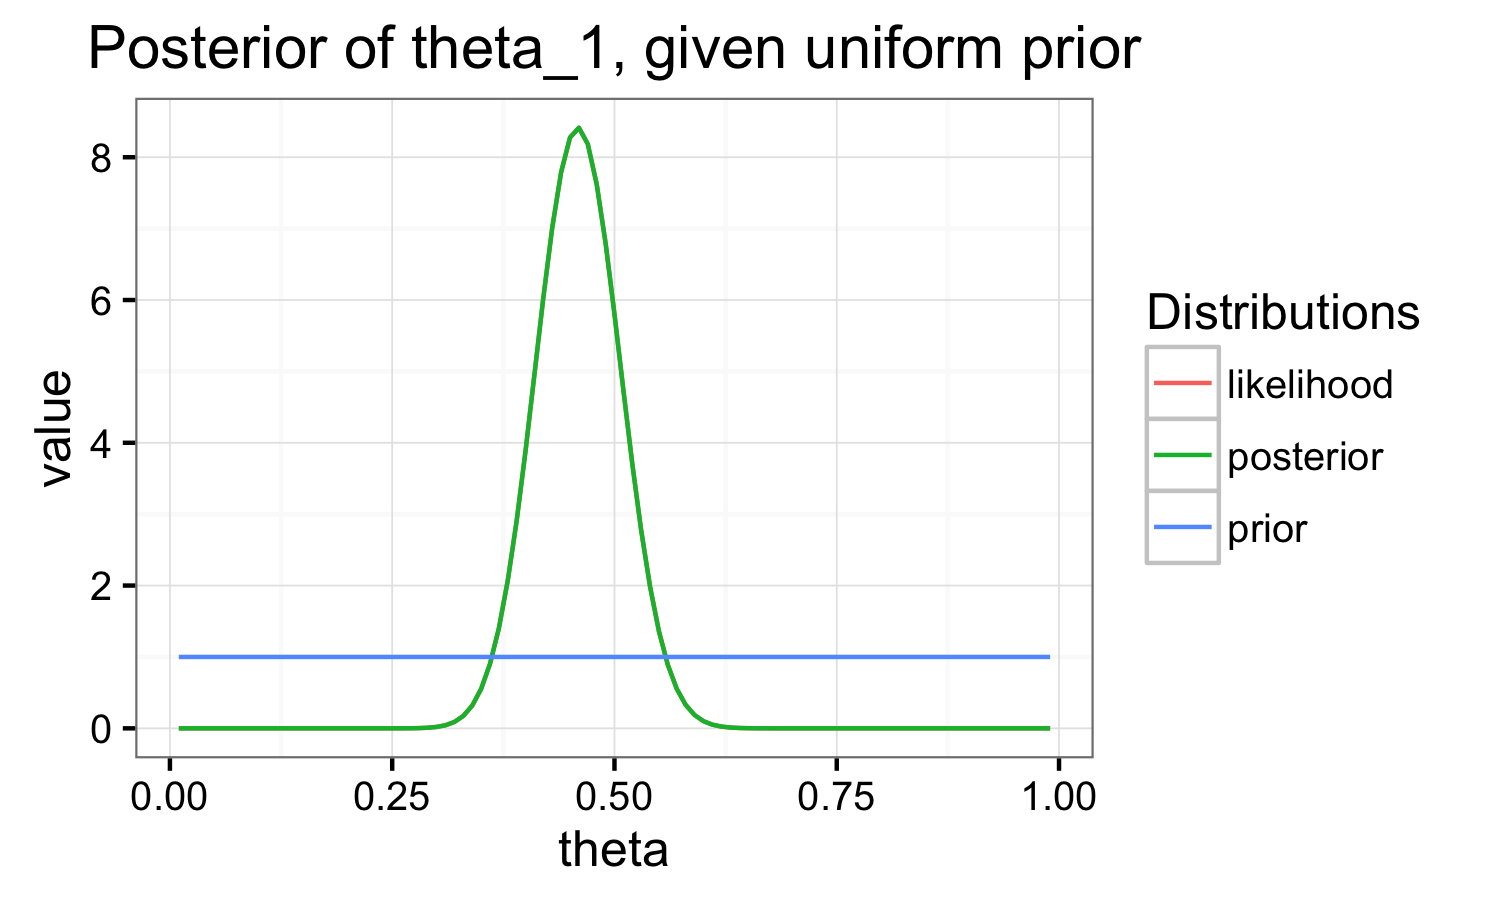
\includegraphics[scale=.18]{11_Assignment1/theta1_c1_posterior.png}
    \caption{Likelihood, prior and posterior distribution of $\theta_1$ given an uniform prior.}
    \label{fig:fig2}
\end{figure}

\begin{figure}[ht!]
    \centering
    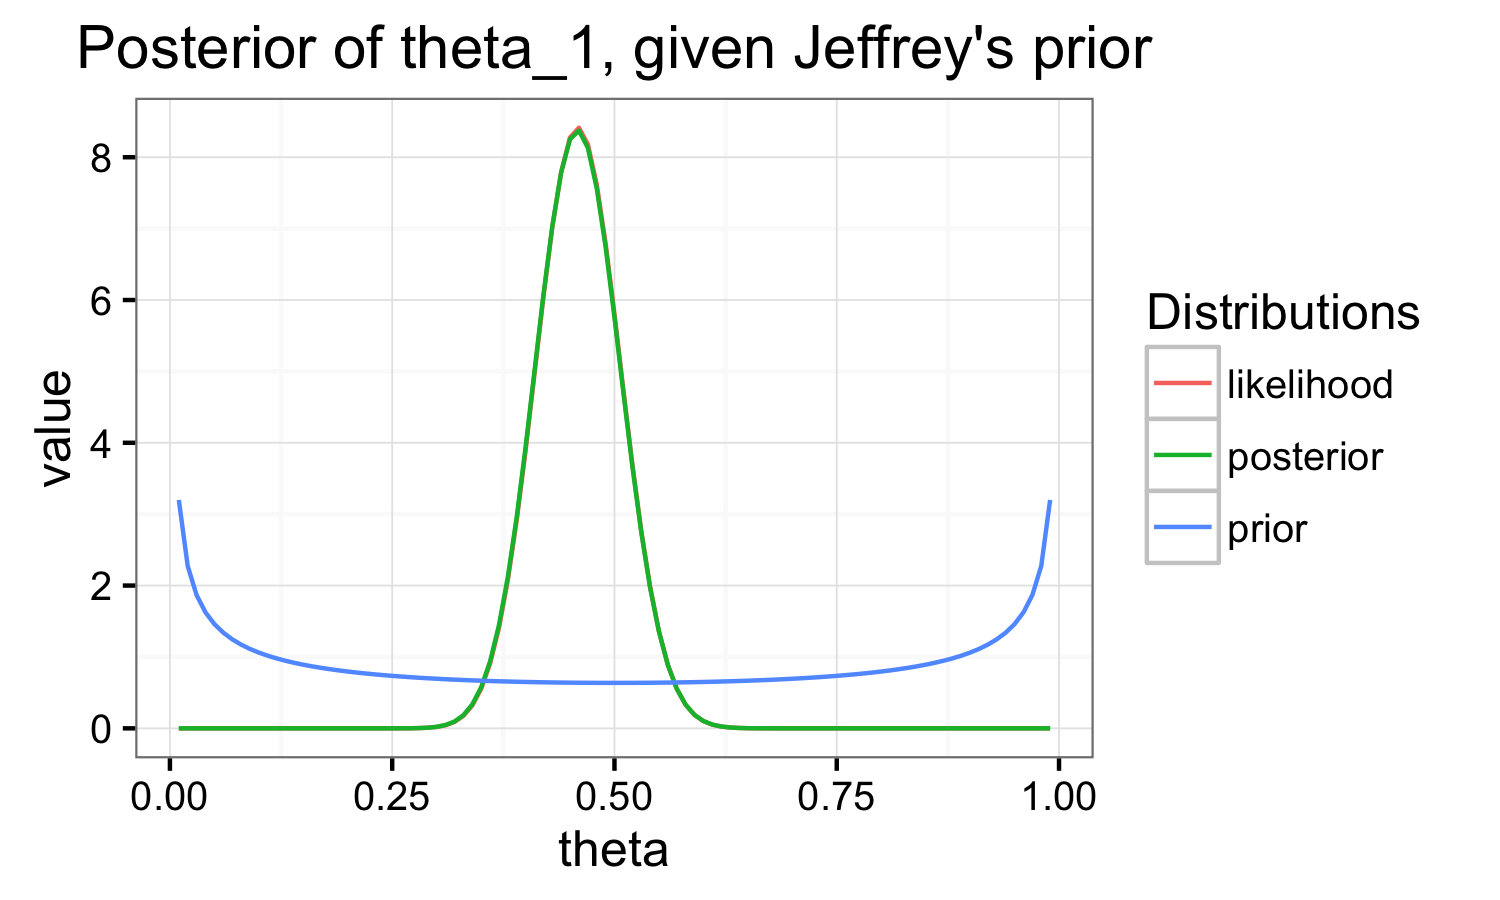
\includegraphics[scale=.18]{11_Assignment1/theta1_c2_posterior.png}
    \caption{Likelihood, prior and posterior distribution of $\theta_1$ given a Jeffrey's prior.}
    \label{fig:fig3}
\end{figure}

\begin{figure}[ht!]
    \centering
    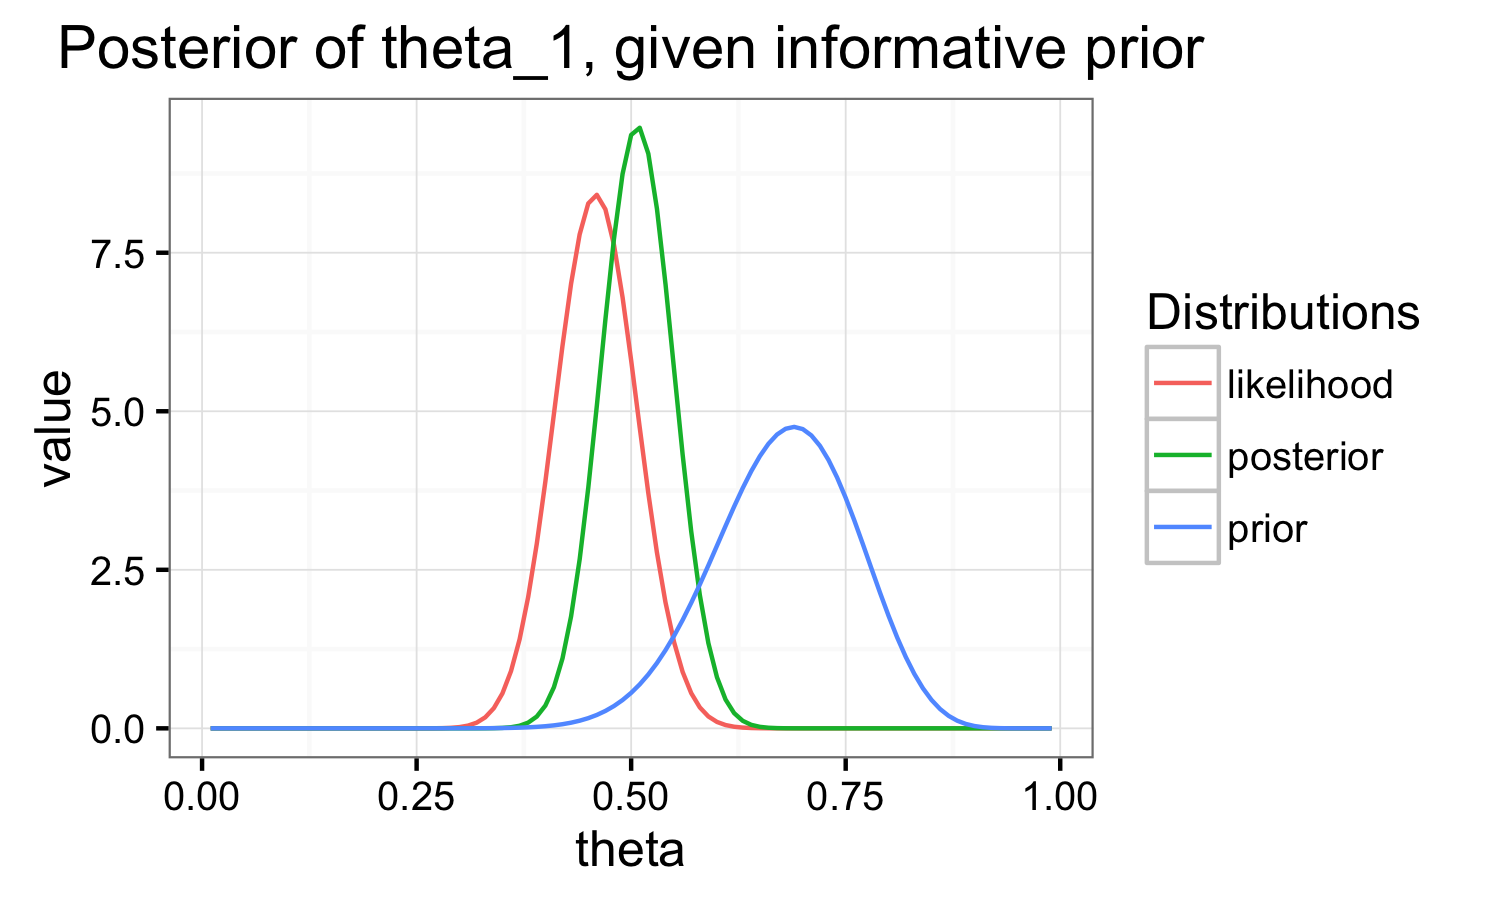
\includegraphics[scale=.18]{11_Assignment1/theta1_c3_posterior.png}
    \caption{Likelihood, prior and posterior distribution of $\theta_1$ given an informative prior.}
    \label{fig:fig4}
\end{figure}

\newpage
With these graphs is easy to see that the first two are very similar. This is because both are created with a non-informative prior. The third one seems that the prior distribution and the likelihood are different (but is closer to the likelihood), so it is possible that the prior is not very correct. In this text, the Jeffrey's prior is the used for the analysis. Below are the equivalent graphs for $\theta_2$ (just 2 non-informative priors were taken).

\begin{figure}[ht!]
    \centering
    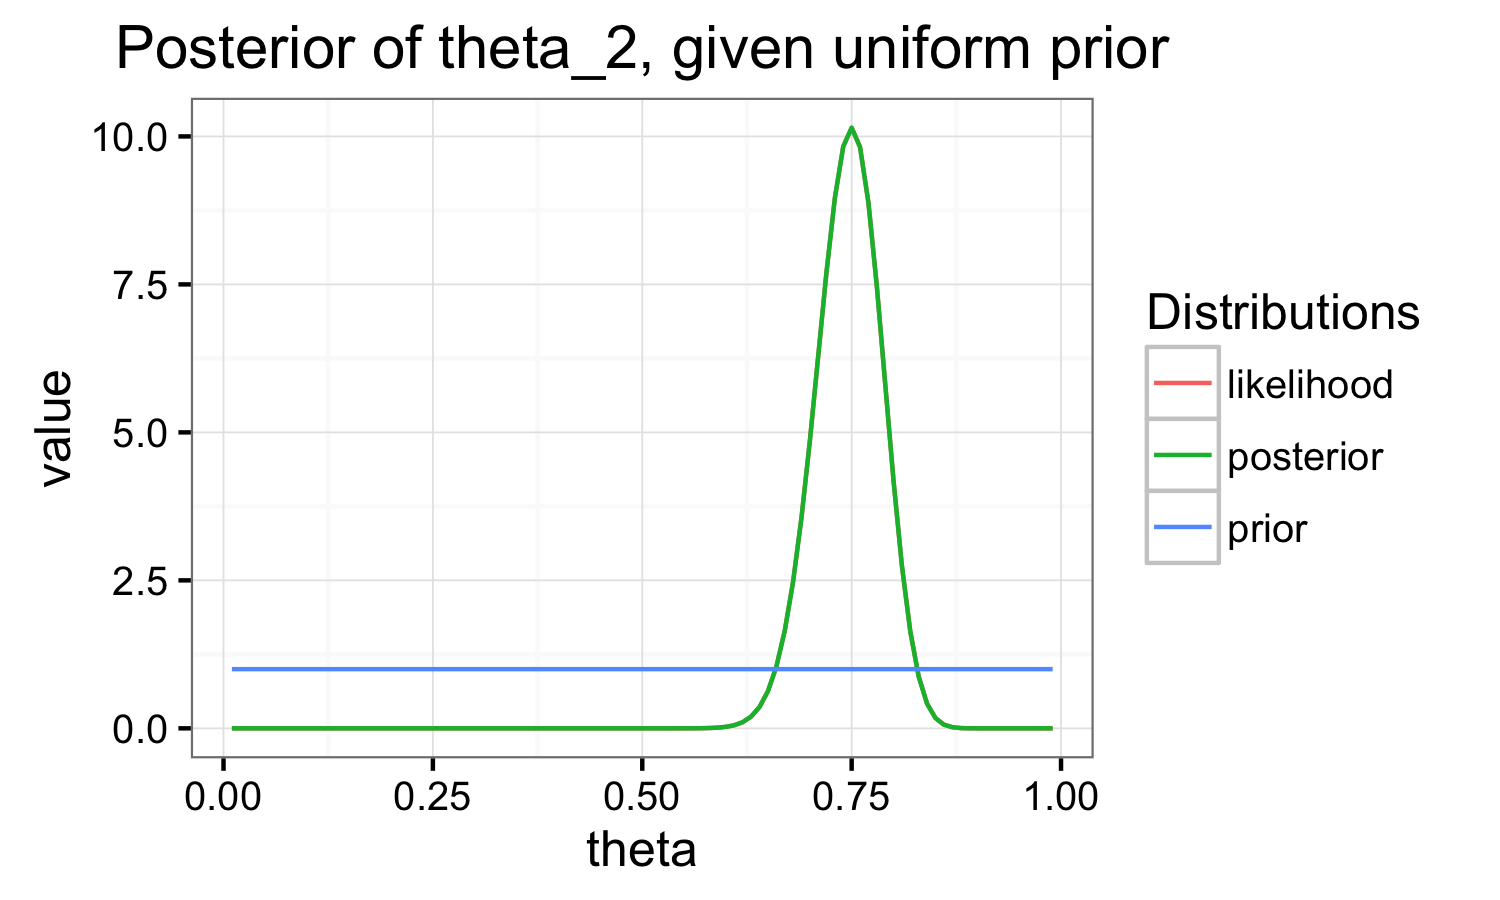
\includegraphics[scale=.20]{11_Assignment1/theta2_c1_posterior.png}
    \caption{Likelihood, prior and posterior distribution of $\theta_2$}
    \label{fig:fig5}
\end{figure}

\begin{figure}[ht!]
    \centering
    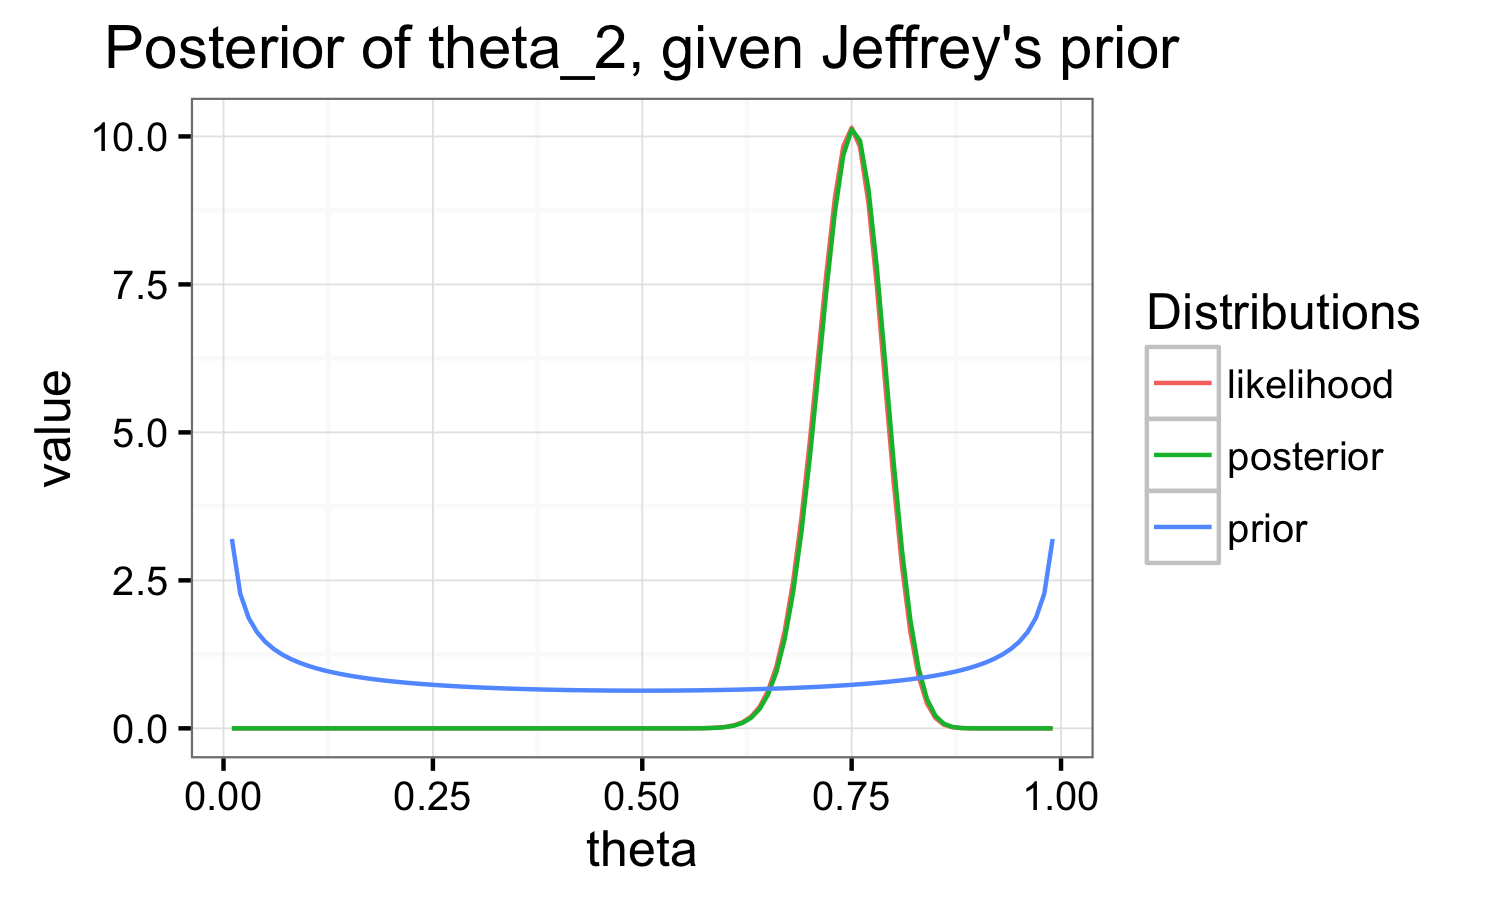
\includegraphics[scale=.20]{11_Assignment1/theta2_c2_posterior.png}
    \caption{Likelihood, prior and posterior distribution of $\theta_2$}
    \label{fig:fig6}
\end{figure}

In the example of $\theta_2$, two non-informative priors were taken, and as can be in the plots above, the distributions are very similar. 

\newpage
\subsection{Posterior predictive summaries and plots}

Now, a comparison of the posterior summaries was made:

\begin{table}[ht]
\centering
\caption{Summary of distributions}
\label{table1}
\begin{tabular}{l|cclll}
Distribution           & \multicolumn{1}{l}{Mean} & \multicolumn{1}{l}{Std} & Median    & CI\_low   & CI\_high  \\ \hline
posterior of $\theta_1$ & 0.4590909                & 4.081275e-05            & 0.4588421 & 0.3984535 & 0.5200510 \\
posterior of $\theta_2$ & 0.7479339                & 2.941329e-05            & 0.7493035 & 0.6966089 & 0.7974833
\end{tabular}
\end{table}

\begin{figure}[ht!]
    \centering
    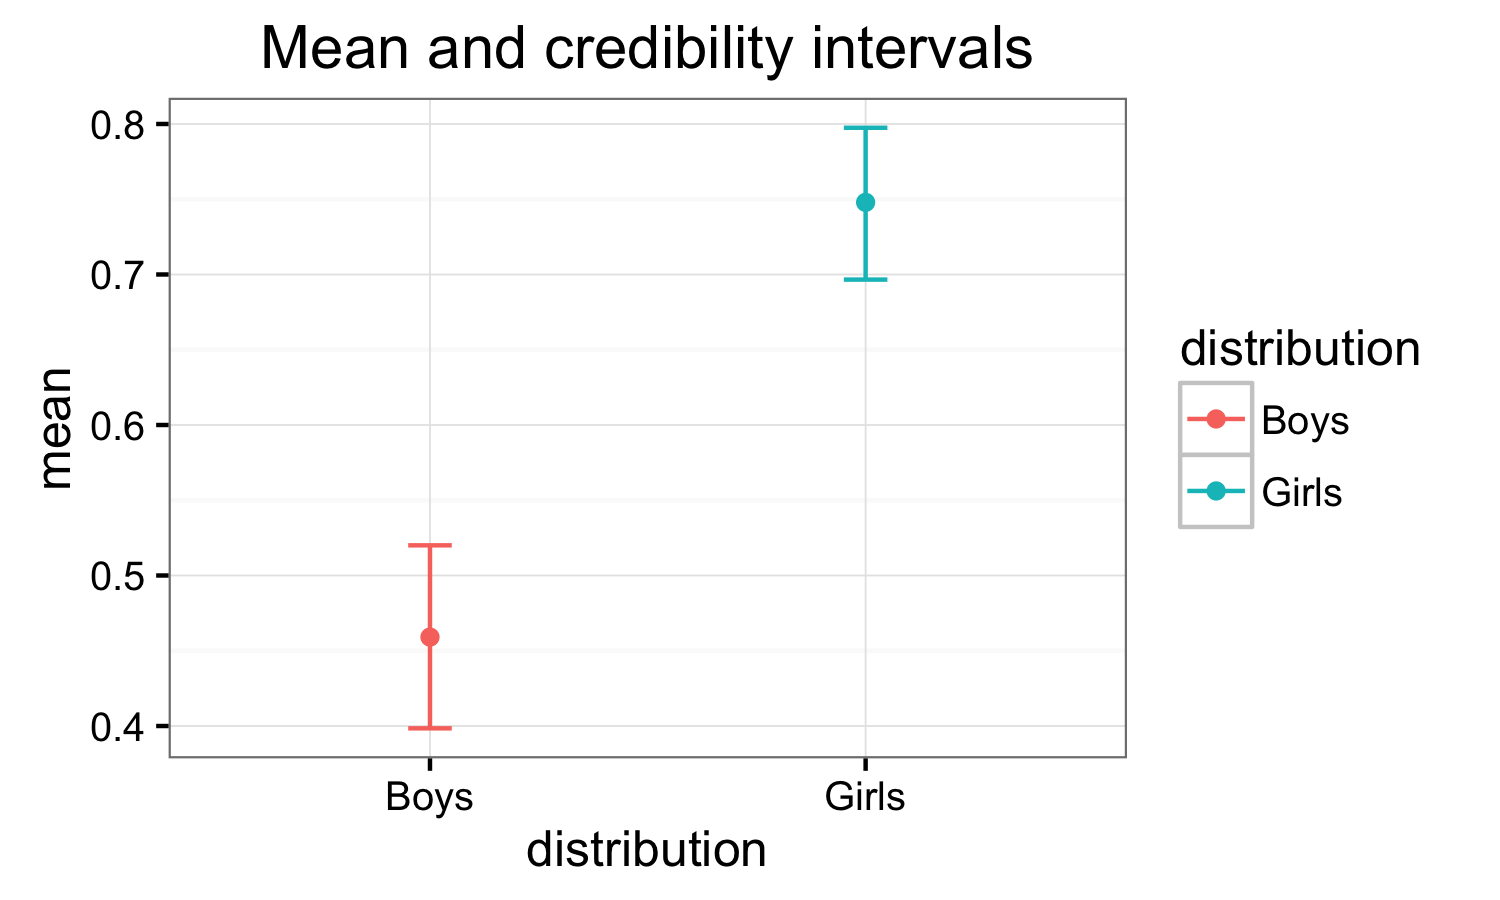
\includegraphics[scale=.20]{11_Assignment1/CI_intervals.png}
    \caption{Credibility intervals of 90\%}
    \label{fig:fig8}
\end{figure}

As can be seen in the two credibility intervals, the difference is big, so it can be concluded that the girls prefer popularity more than boys. Also, the standard deviation of $\theta_2$ is less than the boys. One part of this lower standard deviation could be explained because of the factor of the root square of n that is in its formula.

\subsection{Decisions}

Now, with this graphic is easy to see how different are both posterior distributions:

\begin{figure}[ht!]
    \centering
    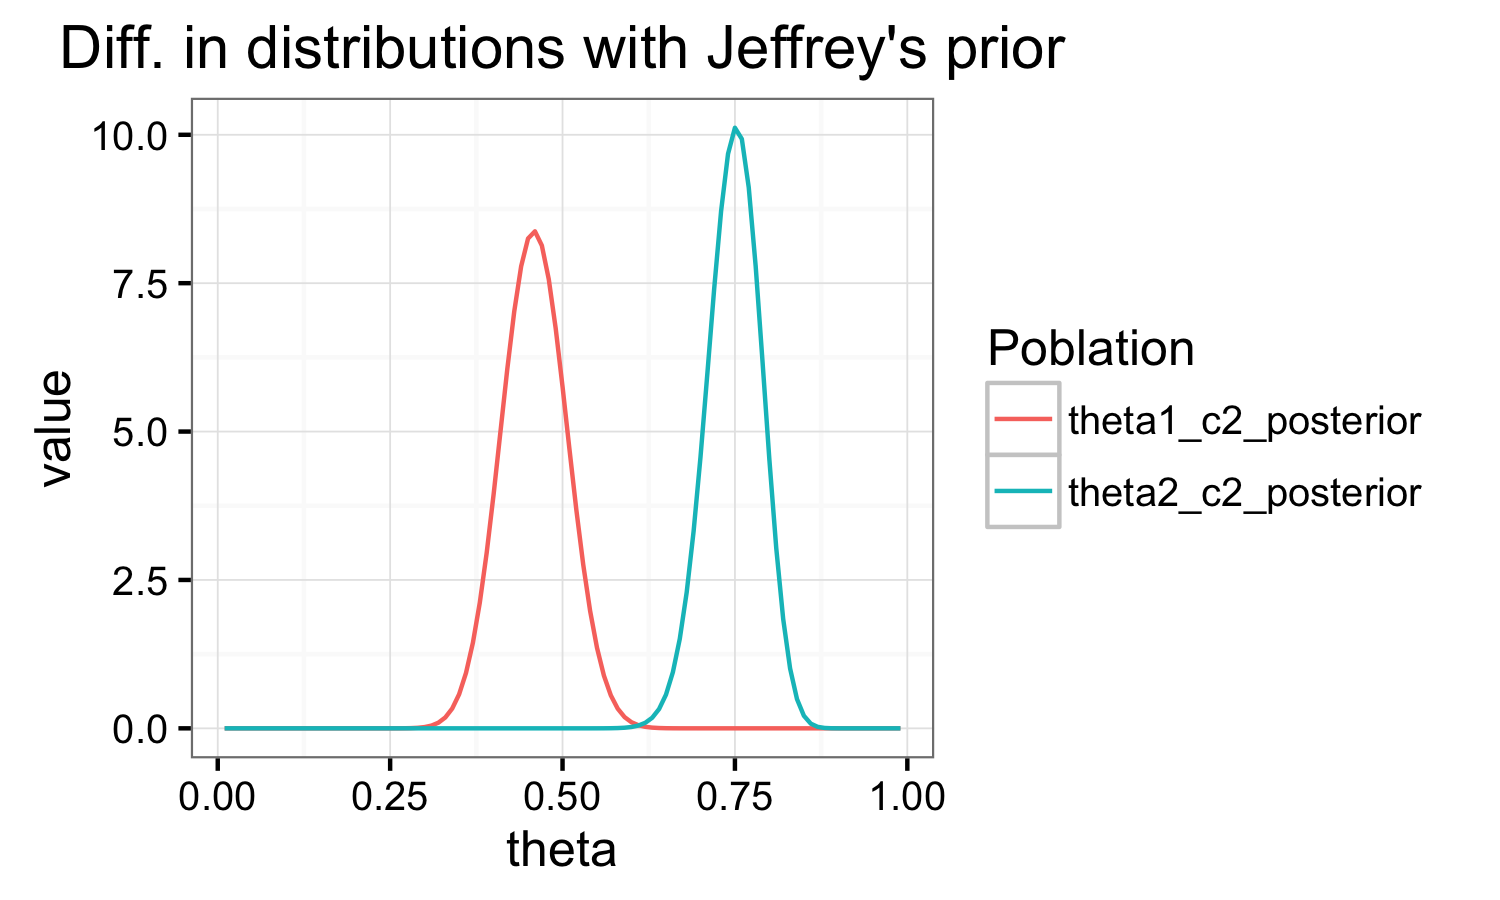
\includegraphics[scale=.20]{11_Assignment1/diff.png}
    \caption{Comparison of posterior distribution of $\theta_1$ and $\theta_2$}
    \label{fig:fig7}
\end{figure}

The assumption that the data is binomial is questionable. Is hard to measure the preferences in a scale of 0-1, because maybe all the people that select $1$ is different and some of them, could prefer much more to be popular than to have sporting ability. For example, a person that is almost indifferent for both decisions should be considered less strong than one that deeply prefers to be popular. For example if the study is made with a 1-5 preference scale, then this differences can be taken into account. This will change completely the distribution of the data. (and maybe this big difference between $\theta_1$ and $\theta_2$ would be smaller!).

\newpage
The independence of each $X_i$ and $Y_i$ can also be questioned. For example, if inside the study there were people that belongs to small groups of friends, then is possible that they think very similar. But this assumption is hard to test if just a $0-1$ variable is given and also without more information. The third thing that could be not a good idea is the use of another prior distribution (at least as the one given). The reason have been stated above.

\section{Conclusions}	

The difference between $\theta_1$ and $\theta_2$ is very big. For example, the 90\% interval of each distribution doesn't overlap. So it is very probable that the $|\theta_1 - \theta_2|$ also doesn't overlap. Given these distributions (and given that both are $\beta$ distributions, is easy to make an hypothesis test (It is not done because is too evident), but can be done. So, with this data, it is easy to conclude that girls prefer more popularity than boys.

\newpage
\appendix

\section{R graphs code}

\lstinputlisting[language=R]
{/Users/salvadorgarcia/Repositories/UoE_2_BDA/11_Assignment1.R}

\end{document}
